\section{Forschungsmethode}
\label{sec:forschungsmethode}

In dieser Arbeit kommt die in der Forschung zu Informationssystemen etablierte Methode von Nunamaker, Chen und Purdin \cite{nunamaker_systems_1990-1} zum Einsatz, die einen strukturierten Rahmen zur Durchführung von Forschungsarbeiten bereitstellt.

\begin{figure}[h]
    \centering
    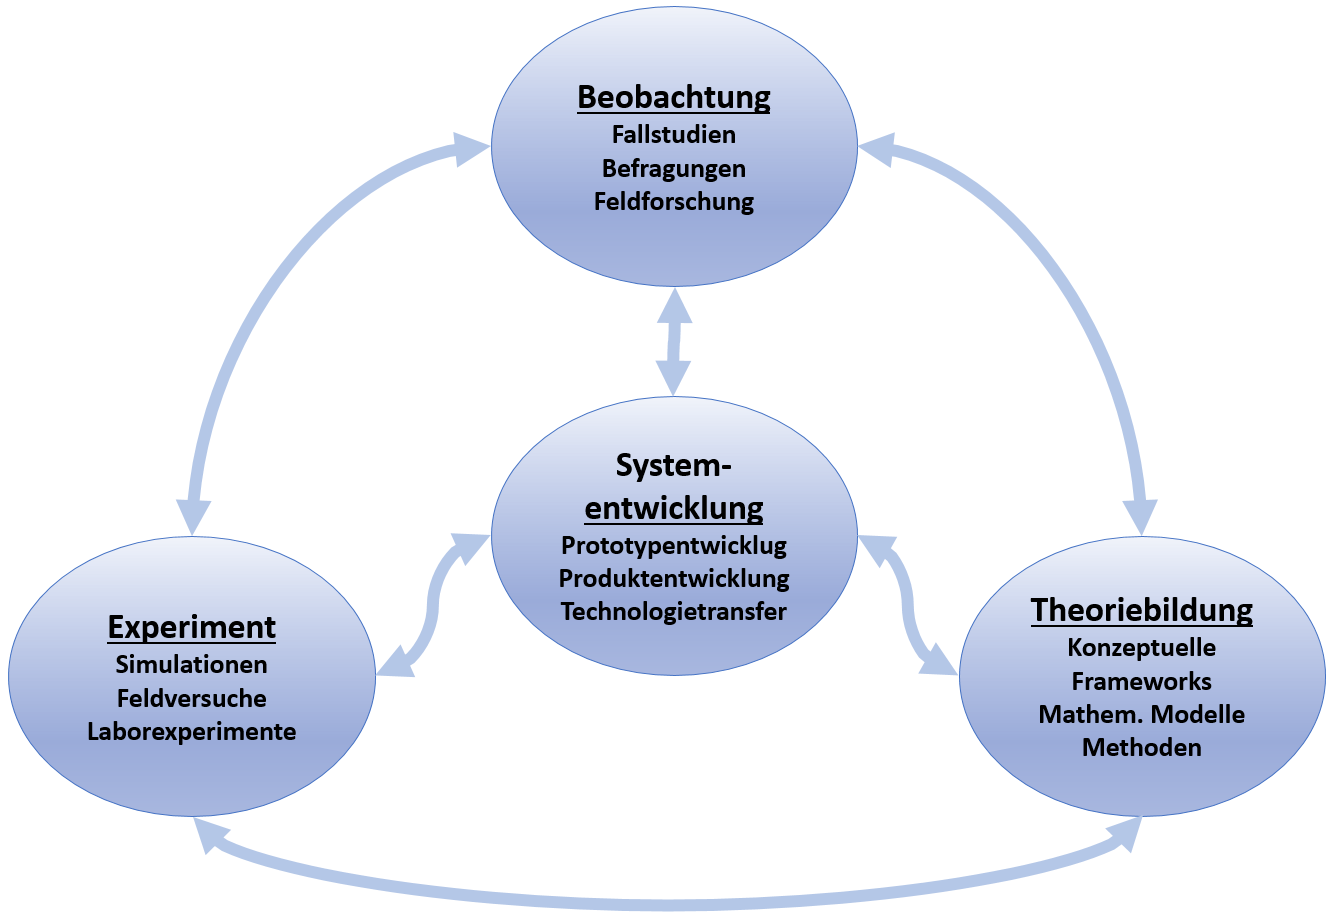
\includegraphics[width=\textwidth]{pictures/Nunamaker2.png}
    \caption{Forschungsmethode nach \cite{nunamaker_systems_1990-1}}
    \label{fig:nunamaker}
\end{figure}

Die Forschungsmethode umfasst die folgenden in Abbildung \ref{fig:nunamaker} dargestellten Phasen:
\begin{description}
\item[Beobachtung:] Insbesondere wenn der Untersuchungsgegenstand relativ unbekannt ist, werden Fallstudien, Feldversuche oder Umfragen durchgeführt, um ein \glqq Gefühl\grqq{} für den Aufwand zu erhalten. Auf dieser Grundlage können dann konkrete Hypothesen erstellt werden, die durch Experimente geprüft werden. 

In dieser Arbeit findet aufgrund der Art des Untersuchungsgegenstandes in der Beobachtungsphase hauptsächlich die Literaturrecherche und Ermittlung des Standes von Wissenschaft und Technik statt.

\item[Theoriebildung:] In dieser Phase werden neue Ideen, Konzepte Methoden oder Modelle entwickelt. Diese Theorien beschreiben das Systemverhalten allgemein, haben jedoch wenig praktische Bedeutung für die Zieldomäne. Sie können aber genutzt werden, um Forschungshypothesen aufzustellen, die Planung von Experimenten zu unterstützen und systematische Beobachtungen durchzuführen.

\item[Systementwicklung:] Diese Phase besteht aus fünf Teilen:
\begin{itemize}
\item Konzeptentwurf

\item Erstellung der Systemarchitektur

\item Erstellung von Prototypen

\item Produktentwicklung

\item Technologietransfer
\end{itemize}


\item[Experiment:] In dieser Phase werden die gefundenen Theorien und entwickelten Systeme evaluiert. Die Ergebnisse der Experimente können genutzt werden, um die Theorien weiterzuentwickeln und die Systeme zu verbessern.

\end{description}

Obwohl die Phasen in der Methode keine vorgegebene Reihenfolge haben, sondern sich gegenseitig beeinflussen, wird in der vorliegenden Arbeit die oben angeführte Abfolge verwendet.

